\section{System Architecture}

\begin{figure}[htb]
\centering
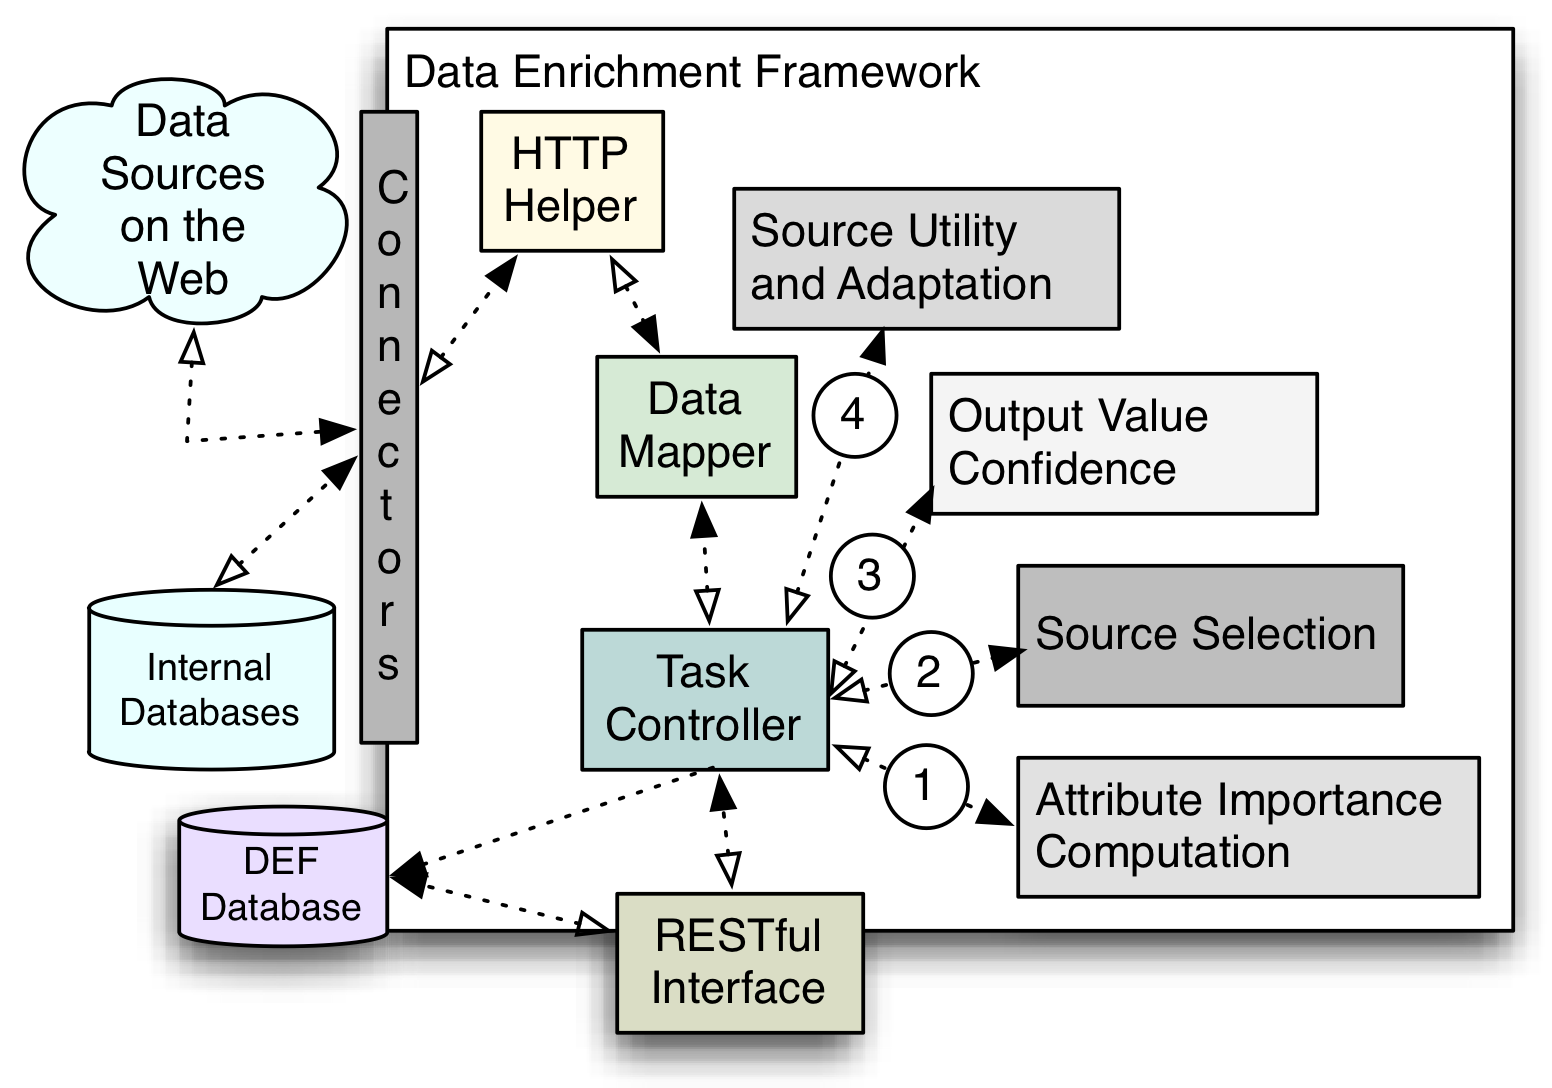
\includegraphics[width=0.45\textwidth]{images/adef_arch.png}
\caption{Overview of Enrichment Algorithm}
\label{fig:overview}
\end{figure}

Figure \ref{fig:overview} illustrates the overview of the enrichment algorithm\footnote{We do not describe the details in this paper. Please visit http:// to get additional information}. The task manager starts a new enrichment project by instantiates and executes the enrichment engine.
The enrichment engine uses the attribute computation module to calculate the attribute relevance. The relevance scores are used in source selection. Using the HTTP helper module, the engine then invokes 
the connector for the selected data source. A connector is a proxy that communicates with the actual data source and is a RESTful Web service in itself. The enrichment framework requires every data source to have a connector and 
that each connector have two operations: 1) a return\_schema GET operation that returns the input and output schema, and 2) a get\_data POST operation that takes as input the input for the data source as POST parameters and returns 
the response as a JSON. For internal databases, we have special connectors that wrap queries as RESTful end points. 
Once a response is obtained from the connector, the enrichment engine computes the output value confidence, applies the necessary mapping rules, and integrates the response with the existing data object. In 
addition to this, the source utility is also computed. The mapping, invocation, confidence and source utility value computation steps are repeated until either all values for all attributes are computed or if all sources
have been invoked. The result is then written into the enrichment database.  

In designing the enrichment framework, we have adopted a service oriented approach, with the goal of exposing the enrichment framework as a ``platform as a service''. 
The core tasks in the framework are exposed as RESTful end points. These include end points for 
creating data objects, importing datasets, adding data sources, and for starting an enrichment task. When the ``start enrichment task'' task resource is invoked and a task is successfully started, the framework responds with a JSON 
that has the enrichment task identifier. This identifier can then be used to GET the enriched data from the database. The framework supports both batch GET and streaming GET using the comet \cite{comet} pattern. 

Data mapping is one of the key challenges in any data integration system. While extensive research literature exists for automated and semi-automated approaches for mapping and matching \cite{mapping1,mapping2}
it is our observation that these techniques do not guarantee the high-level of accuracy required in enterprise solutions. So, we currently adopt a manual approach, aided by a graphical interface for data mapping. The source and 
the target schemas are shown to the users as two trees, one to the left and one to the right. Users can select the attributes from the source schema and draw a line between them and attributes of the target schema. Currently, our
mapping system supports assignment, merge, split, numerical operations, and unit conversions. When the user saves the mappings, the maps are stored as mapping rules. Each mapping rule is represented as a tuple containing the 
source attributes, target attributes, mapping operations, and conditions. Conditions include merge and split delimiters and conversion factors.  


